\documentclass[12pt,a4paper]{book}
\usepackage[labelsep=endash]{caption}
\usepackage[utf8x]{inputenc} %использование кодировки Юникод UTF-8
\usepackage[russian]{babel} %пакет поддержки русского языка
%\usepackage{russianb}


\usepackage{indentfirst}
\setlength{\parindent}{0.75cm}

\usepackage{amsmath}
\usepackage{amssymb}
\usepackage{graphicx}
\usepackage[labelsep=endash]{caption}
\usepackage{subcaption}
\usepackage{listings}

\usepackage[compact]{titlesec}
\titlespacing*{\section}{0.75cm}{1em}{0.1em}
\titlespacing*{\subsection}{0.75cm}{1em}{0.1em}
%\chapter[\CYRO\cyrd\cyrn\cyro\cyrsh\cyra\cyrg\cyro\cyrv\cyrery\cyre~\cyra\cyrl\cyrg\cyro\cyrr\cyri\cyrt\cyrm\cyrery]{Одношаговые алгоритмы}

\begin{document}
\setcounter{chapter}{1}
%\chapter{Одношаговые алгоритмы численного интегрирования}
\chapter[\CYRO\cyrd\cyrn\cyro\cyrsh\cyra\cyrg\cyro\cyrv\cyrery\cyre~\cyra\cyrl\cyrg\cyro\cyrr\cyri\cyrt\cyrm\cyrery]{Одношаговые алгоритмы}
\section{Неявные методы Рунге-Кутты}
\setcounter{subsection}{1}
\subsection{Жесткие задачи. Понятия А-устойчивости и L-устойчивости}

С самого начала применения численных методов обнаружилось, что с их помощью не всегда удается получить решение дифференциальных уравнений: иногда эти методы давали расходящийся процесс, хотя точные решения уравнений были заведомо сходящимися.  Ч. Кёртисс  и Дж. Хиршфельдер в знаменитой работе «Интегрирование жестких уравнений» [1] 1952 года ввели понятие жесткости для таких дифференциальных уравнений (в дальнейшем предлагались иные математические формулировки этого термина; общепризнанного определения до сих пор нет). Жесткими могут быть уравнения, описывающие образование свободных радикалов в сложной химической реакции (пример Кертисса и Хиршфельдера $ \dot{x} = 5(x-t^{2}) $ , «брюселлятор»), диффузию, колебаний упругого стержня и др. Динамическая система, описываемая жесткими уравнениями, также называется жесткой. Свойства жесткости и метода, пригодного для решения жестких уравнений, наглядно демонстрирует оригинальная иллюстрация из статьи Кертисса и Хиршфельдера (рис. \ref{fig:methodprop}). Здесь $ Y(x) $  истинное решение уравнения; непригодный для жестких систем метод приводит к уклонению приближенного решения от истинного и уходу его в плюс или минус бесконечность в зависимости от константы итегрирования $ C $. Пригодный для жестких систем метод дает сходящееся к $ Y(x) $  решение (пунктирная линия) независимо от того, из какой точки $ (y_0,x_0) $  он стартует. 
 
 \setcounter{figure}{6}
\begin{figure}[h!]
 	\centering
 	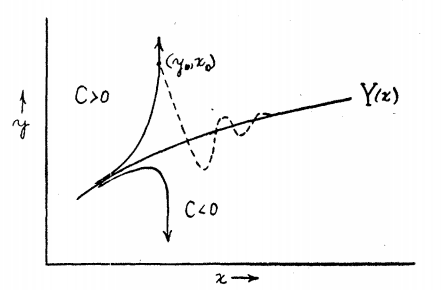
\includegraphics[width=0.7\linewidth]{method_prop}
 	\caption{Свойства метода, пригодного для решения жестких систем.}
 	\label{fig:methodprop}
\end{figure}
\newpage
 
%Рис. 2.7 ? Свойства метода, пригодного для решения жестких систем. 
Хайрер, Нерсетт и Ваннер [3] объясняют явление жесткости на примере задачи

\setcounter{equation}{31}
\begin{equation}
\dot{x} = -50(x-cost)
\label{for}
\end{equation}

графики решения которого представлены на рис. \ref{fig:eulers}.  Вблизи $ x \approx cost $  имеется медленно изменяющееся решение, а другие решения подходят к нему после быстрой «переходной фазы». Такие быстрые переходы типичны для жестких уравнений, но не являются ни достаточным, ни необходимым их признаком: так, у решения с начальным значением $ x(0) = 2500/2501 $  нет переходной фазы. На рис. \ref{fig:eulers} справа приведен график решения методом Эйлера для начального значения $ x(0) = 0 $  и длин шагов $ h = 1,974/50 $  и $ h = 1,875/50 $ . Как только длина шага становится немного больше критической величины, численное решение уходит слишком далеко за равновесное, и возникают все более сильные колебания, отсутствующие в точном решении уравнения.

\begin{figure}[h!]
	\centering
	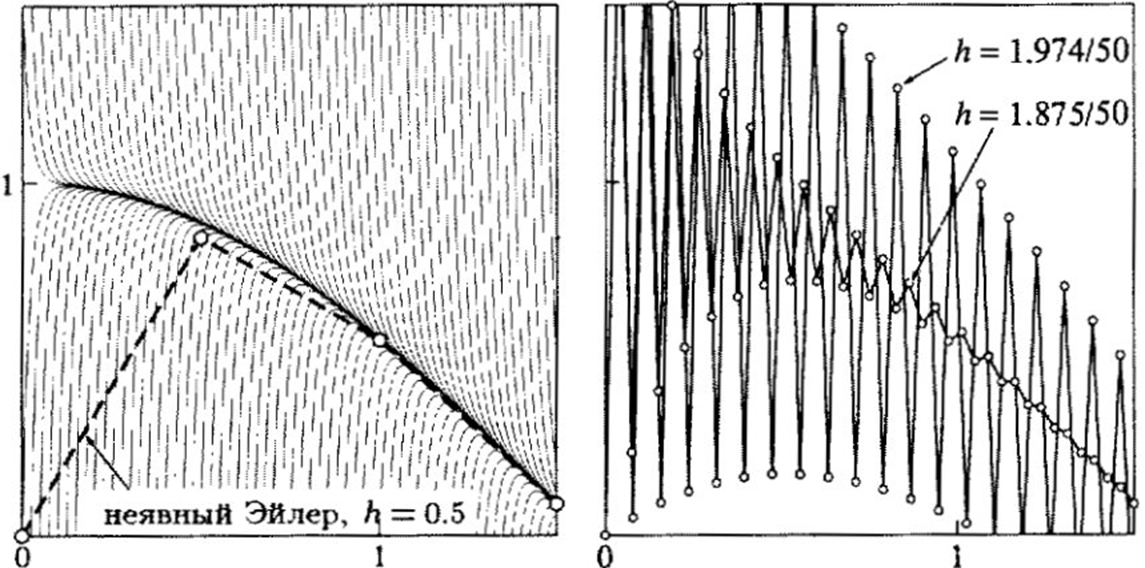
\includegraphics[width=0.7\linewidth]{eulers}
	\caption[eur]{Кривые решения уравнения (\ref{for}) [1]}
	\label{fig:eulers}
\end{figure}
\newpage
%Рис. 2.8 – Кривые решения уравнения (2.32) [1]
Первоначально понятие жестких уравнений вызывало скепсис, так как считалось, что это очень частный случай, однако, по словам Г. Далквиста, «около 1960 года положение изменилось и все осознали, что мир полон жестких задач» [2].
Исследование свойств методов, пригодных для решения жестких уравнений, привело к возникновению понятия абсолютной устойчивости, или А-устойчивости (введено Г. Далквистом в 1963 г.). Метод называется А-устойчивым, если для любых собственных чисел $\lambda $, $ у $ которых $ Re(\lambda)<0 $, и любого шага интегрирования при решении линеаризованного уравнения

\begin{equation}
\dot{x} = \lambda x
\label{for2}
\end{equation}

он дает сходящееся решение [3]. Было выдвинуто предположение, что методы, пригодные для решения жестких систем, должны быть А-устойчивыми. 
\end{document}